As mentioned in the Methodology section~\ref{sec:methodology}, the first step was to analyse time series the anemometers and thermocouples averaged in a 30 minute period. 

In the top panel shows the CSAT3 air temperature and the ground temperature measurements. At first glance is possible to see that there is a gap in the data between the 17th and the 19 of February when none of the CSAT3 instruments were measuring. In the lower panel, we can see the time series of the Thermocouples. They follow a similar variation as the CSAT3 instruments, but they were recording during the whole campaign. 

\begin{sidewaysfigure}
  \centering
  {
  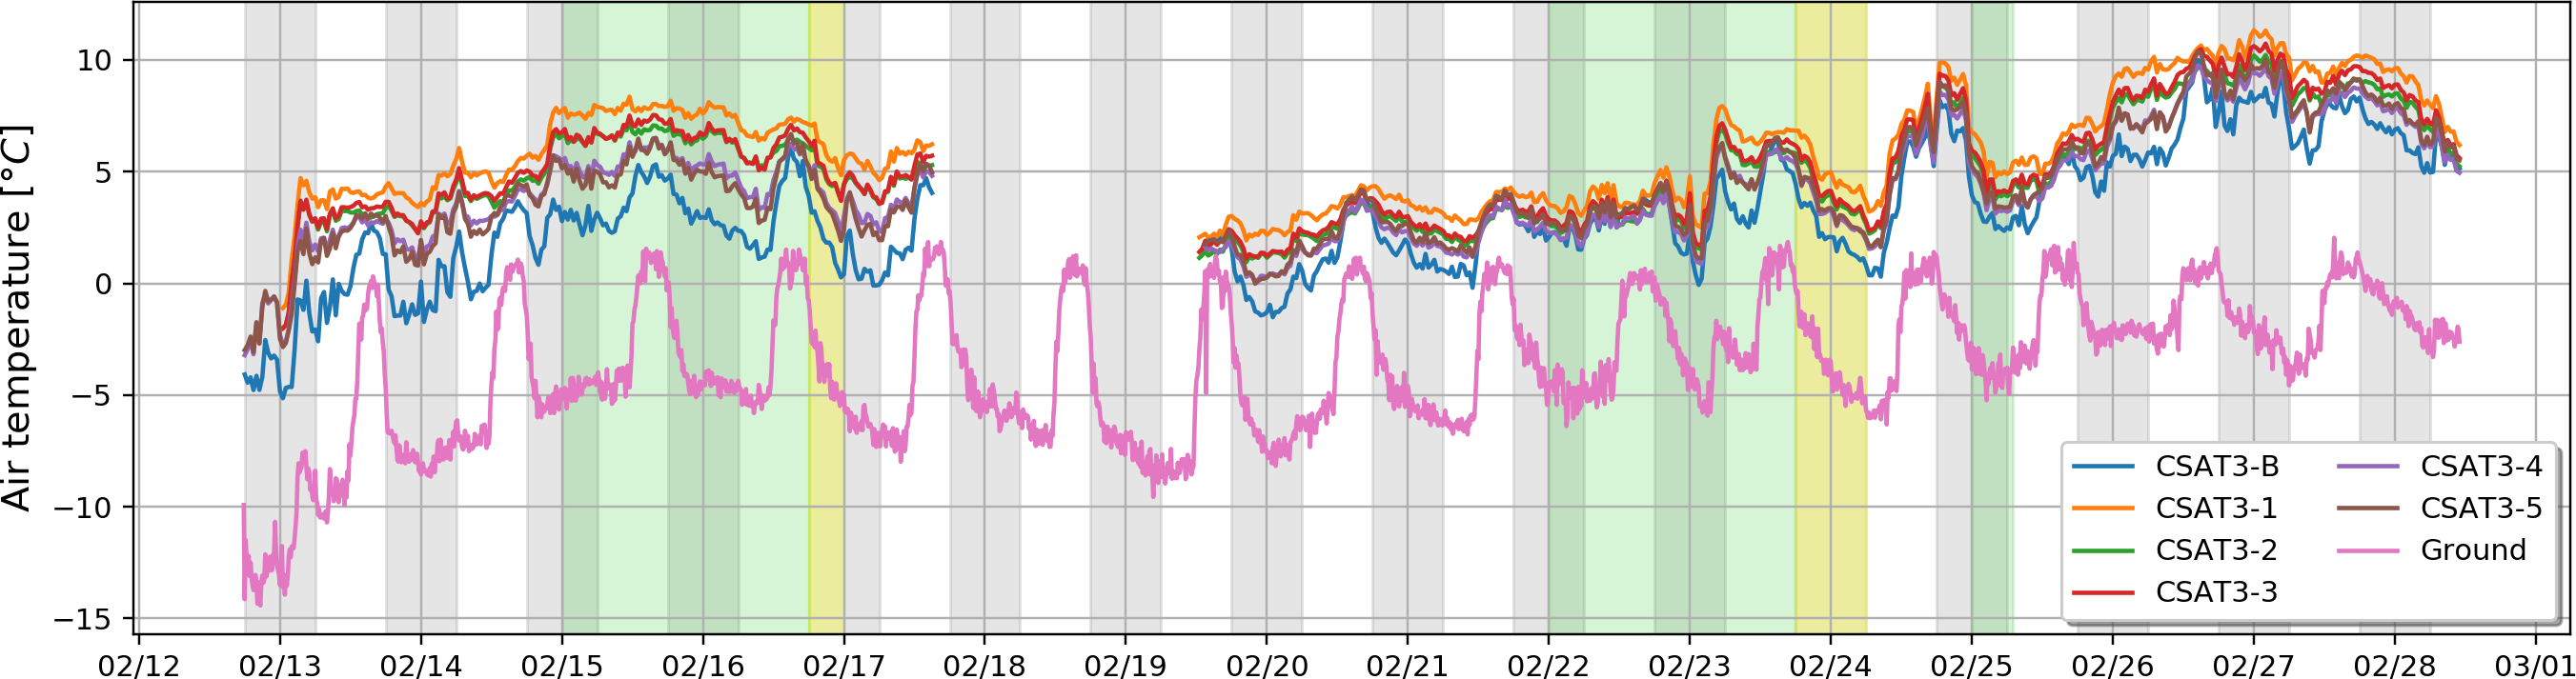
\includegraphics[width=1\textwidth]{fig/chapter_4/csat_temp_series.png}\\
   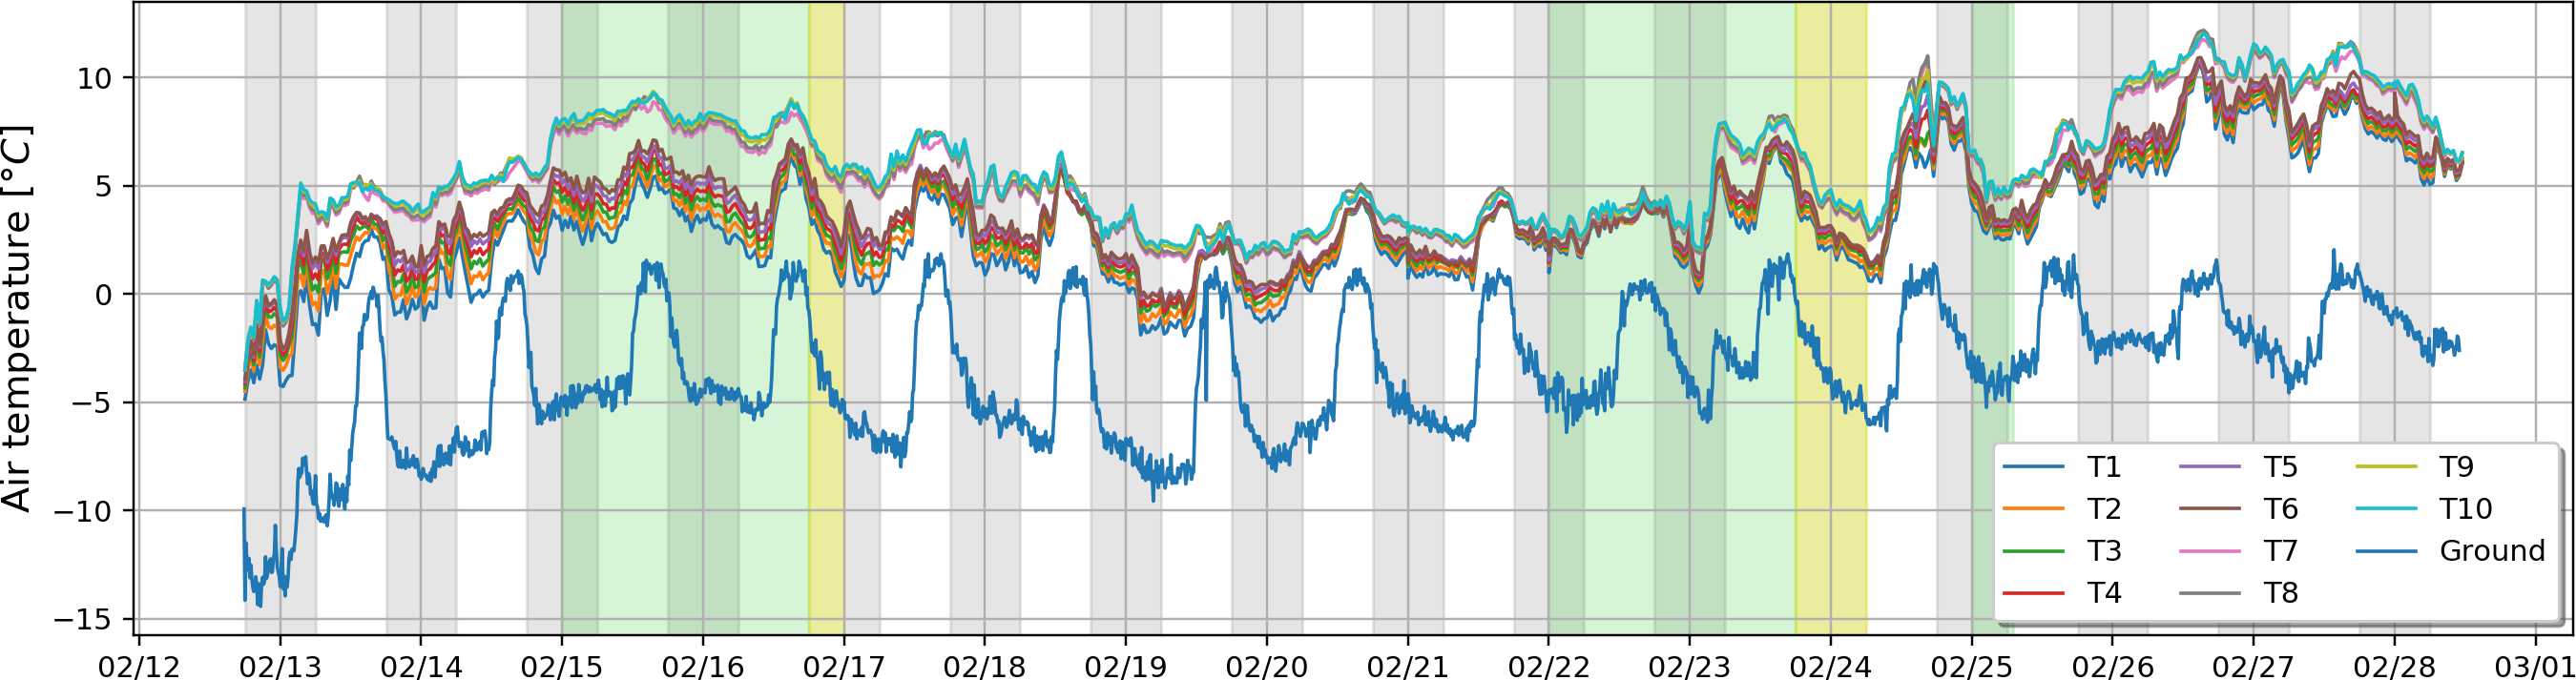
\includegraphics[width=1\textwidth]{fig/chapter_4/TC_temp_series.png}
   }
  \caption{Time series of air temperature of the whole field campaign. The top panel shows the air temperature recorded by the CSAT3 instruments and the lower panel the air temperature recorded with the Thermocouples. In both figures, the grey shadows represent the night periods, the green shadows the favourable days from in situ observation and the yellow shadows the nights chosen for the analysis. Both plots have the ground temperature as a reference point.}
  \label{fig:temp_series}
\end{sidewaysfigure}

In figure~\ref{fig:windspeed_series} the time series (30 minutes average) of the wind speed of the CSAT3 and the Windsonic anemometers are shown. The top panel corresponds to the CSAT3's, where is possible to see the gap of the data in the middle of the campaign. The lower panel corresponds to the Windsonic 2-D instruments, where we can see that during the beginning of the campaign (from the 12th to the 19th) only the Winsonic No.0 and No.1 were working. From the 19th until the end of the campaign, the four Windosinc were working. 

\begin{sidewaysfigure}
  \centering
  {
  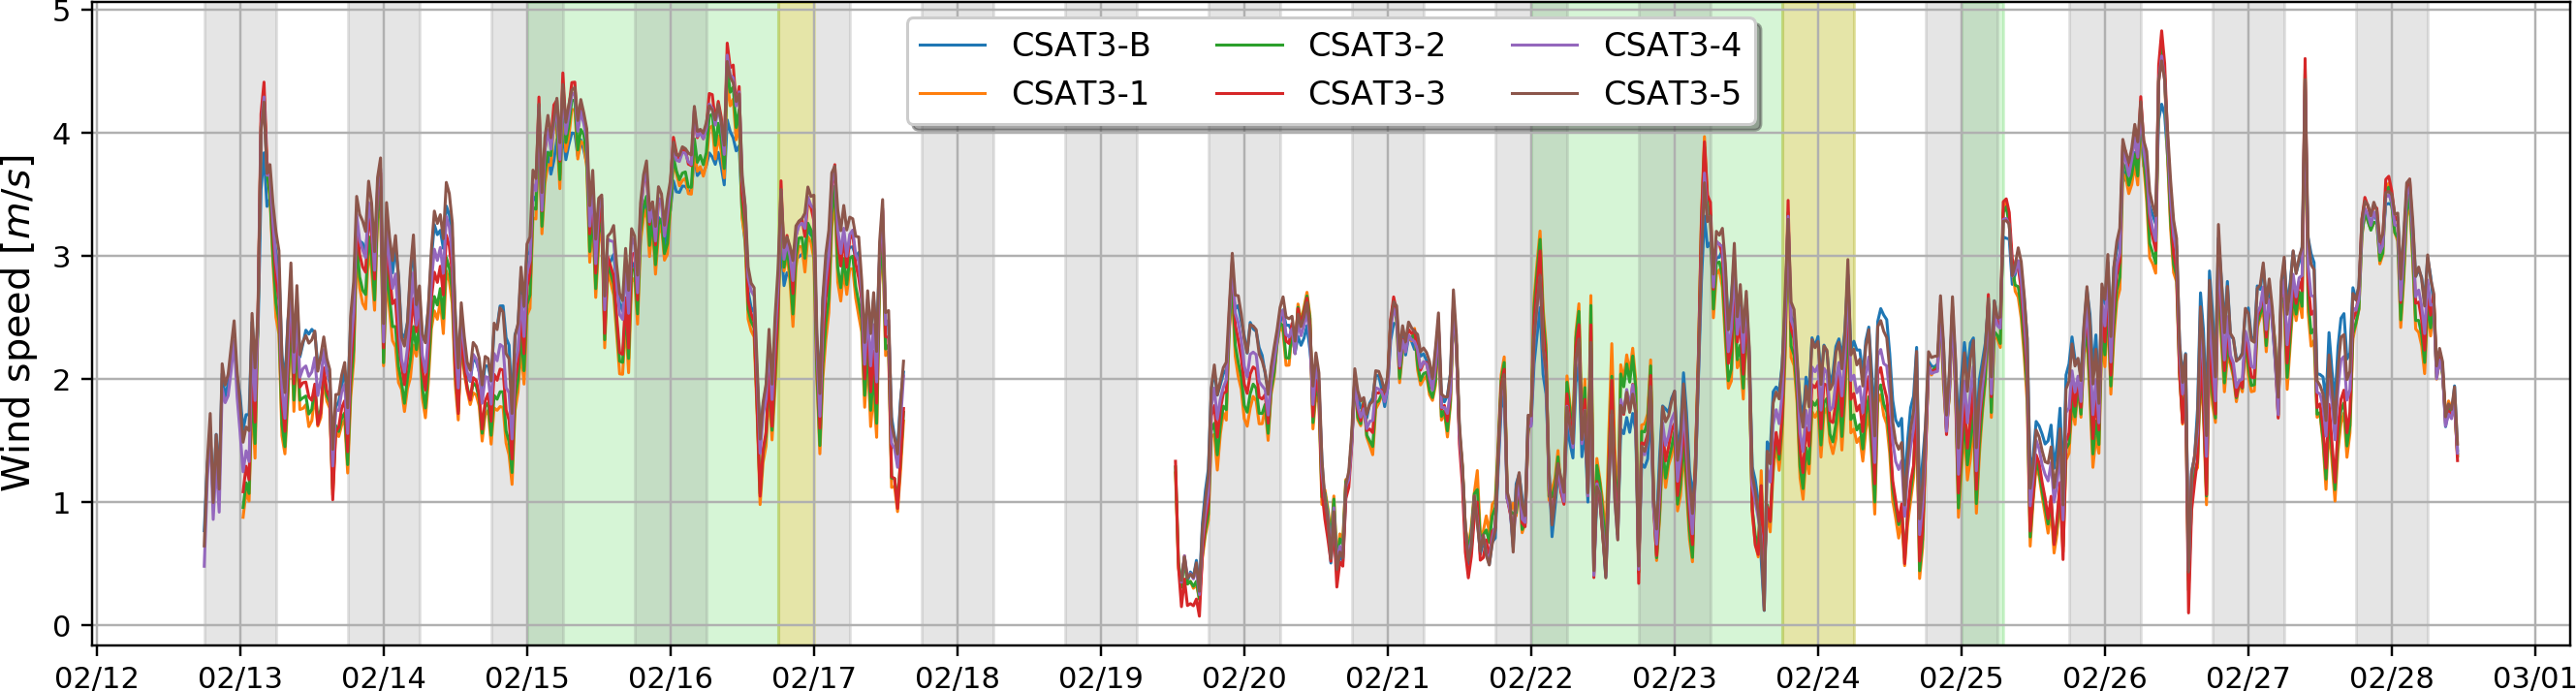
\includegraphics[width=1\textwidth]{fig/chapter_4/wind_speed_csat_series.png} \\
   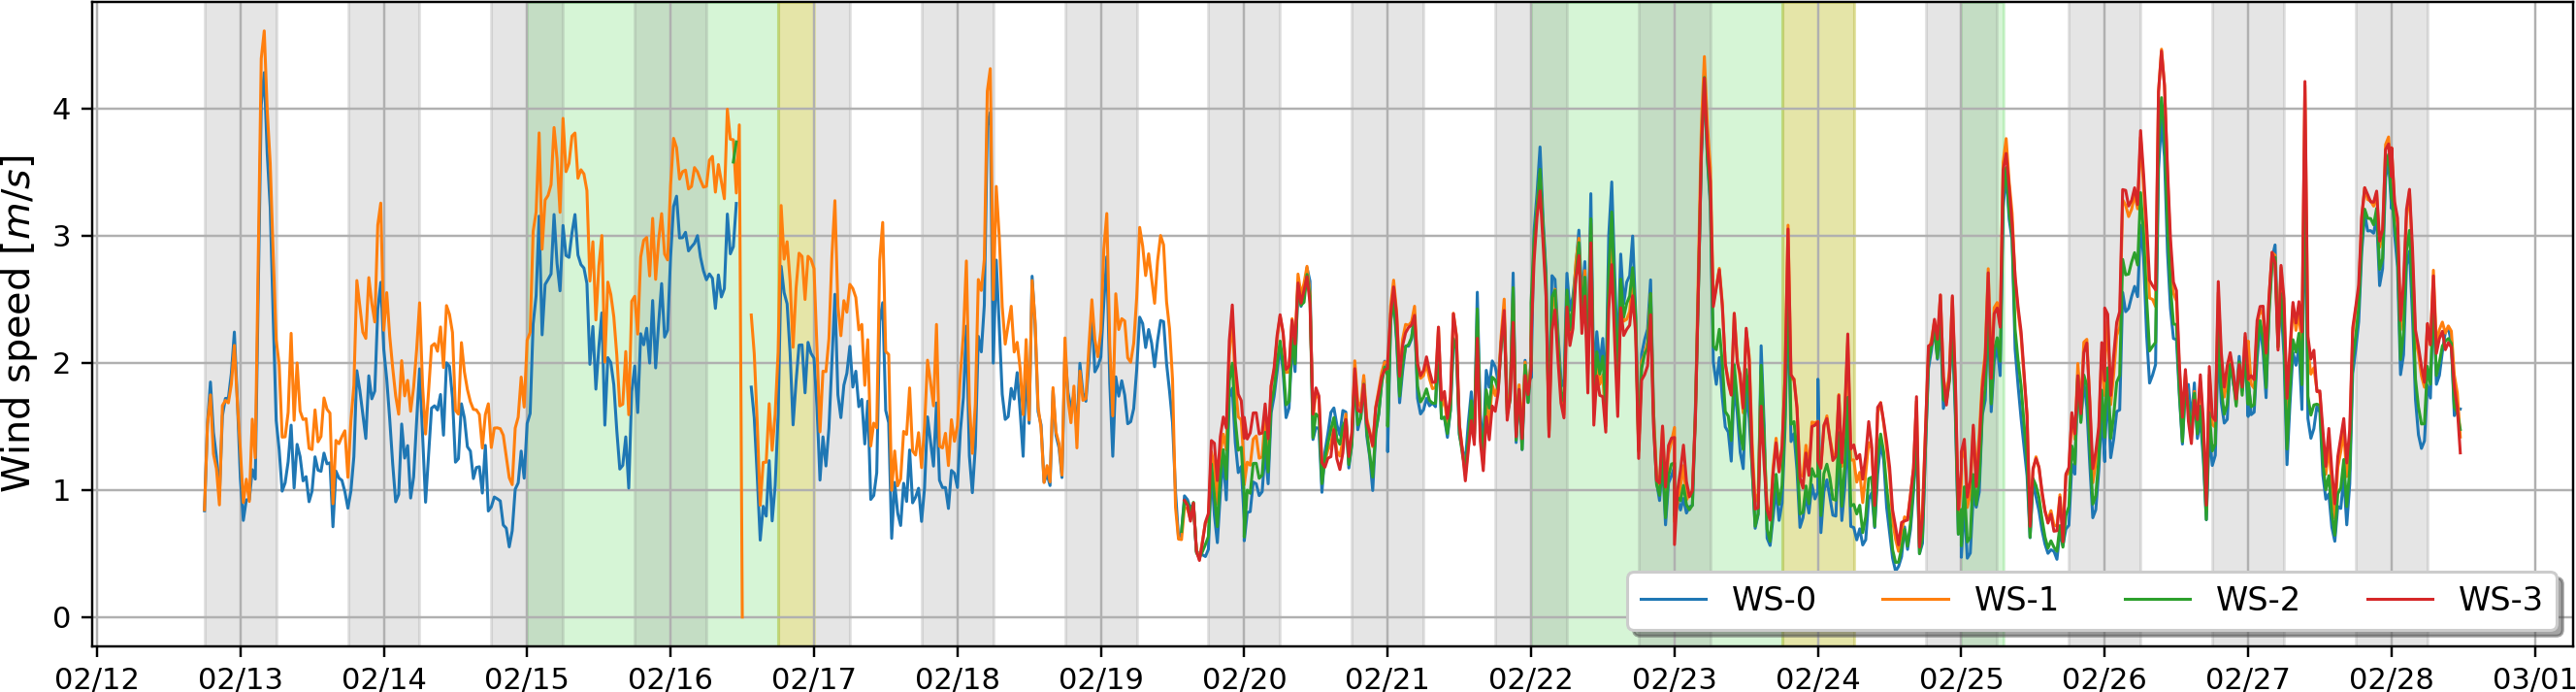
\includegraphics[width=1\textwidth]{fig/chapter_4/wind_speed_ws_series.png}
   }
  \caption{Time series of wind speed of the whole field campaign. The top panel shows the wind speed recorded by the CSAT3 instruments and the lower panel the winds speed recorded with the Windsonic 2-D (WS). In both figures, the grey shadows represent the night periods, the green shadows the favourable days from in situ observation and the yellow shadows the nights chosen for the analysis. Both plots have the ground temperature as a reference point.}
  \label{fig:windspeed_series}
\end{sidewaysfigure}

In both figures~\ref{fig:temp_series} and \ref{fig:windspeed_series}, there are periods marked by green and yellow shadows. The green ones indicate the favourable days for the development of katabatic winds, according to the in situ observations. The yellow periods indicate the nights that were selected for the analysis in this work, according to the criteria for choosing a good night. We selected the nights of the 16th to the 17th and the night from the 23rd to the 24th. These were chosen because there was a pronounced drop in the temperature of the ground and the air from the sunset, which is the principal forcing that drives these winds, and they were in the favourable periods to detect these winds.

\section{Calibration}

In figure~\ref{fig:csat1_vs_ws3} we can see a scatter plot comparing the 30 minutes averaged wind speed measured with the wind sonic versus the one measured with the CSAT3-B, with the data of the whole campaign. A linear regression was done to the data, to which it was found that the correlation coefficient ($R = 0.94$).  

\begin{figure}[!ht]
    \centering
    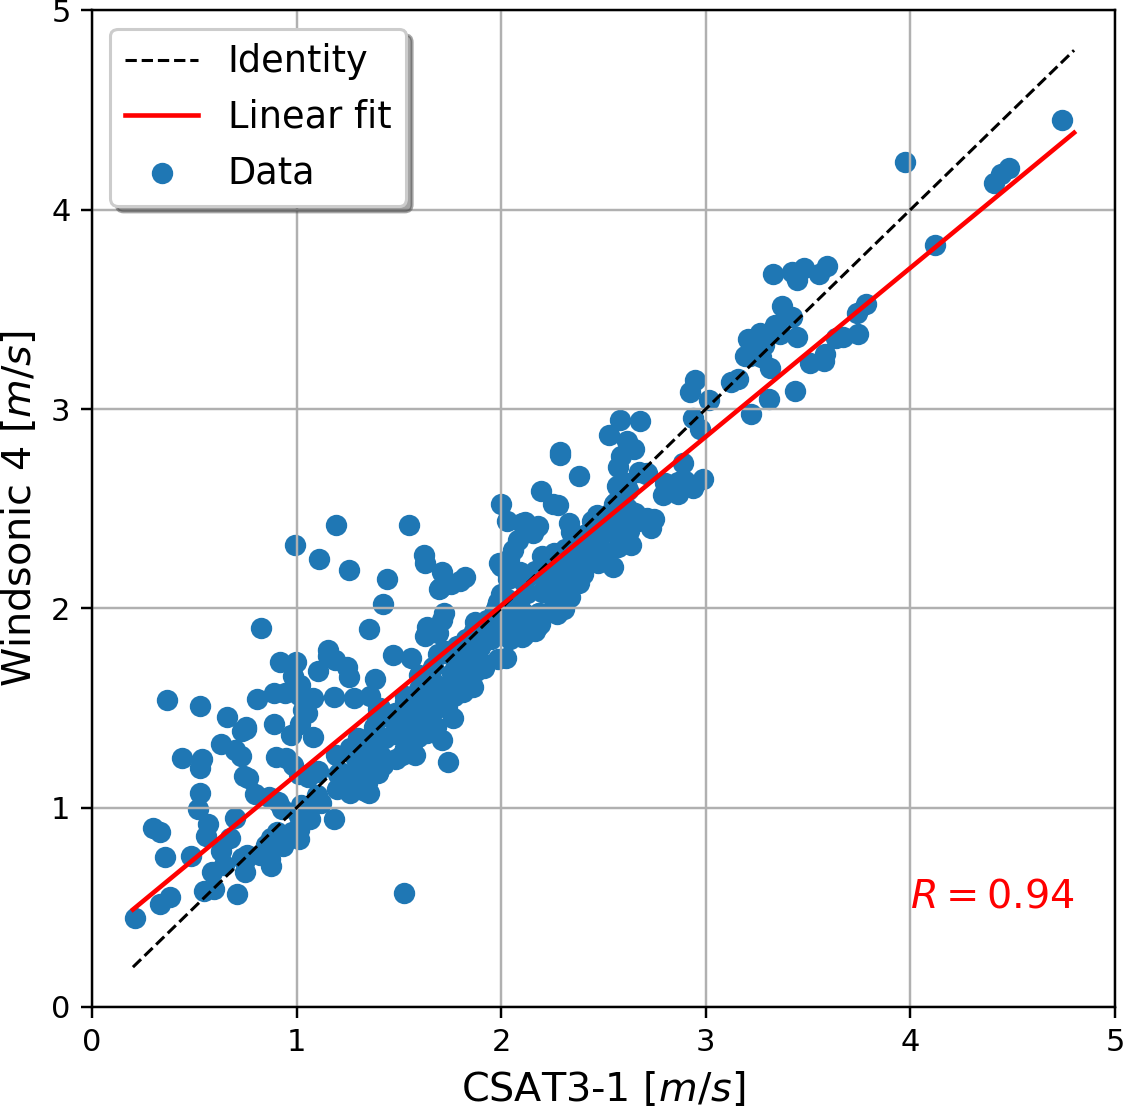
\includegraphics[width=0.48\textwidth]{fig/chapter_4/gunshot_csat1_vs_ws3.png}
    \caption{Scatter plot comparing the wind speeds of the Windsonic 4 and the CSAT3 No.1. The red line is a linear fit done to the data, with a correlation coefficient $R$ of 0.94.}
    \label{fig:csat1_vs_ws3}
\end{figure}

Figure~\ref{fig:csat_vs_TC} shows the comparison of the temperature measured with the CSAT3 and the Thermocouples. In particular, the figure on the left is the comparison between the CSAT3-B and the thermocouple 1, which have a $R = 0.996$. On the right side, the figure compares the CSAT3 No.4 with the Thermocouple 6. The data have a $R = 0.989$. 

\begin{figure}[!ht]
    \centering
    \begin{subfigure}[b]{0.48\textwidth}
        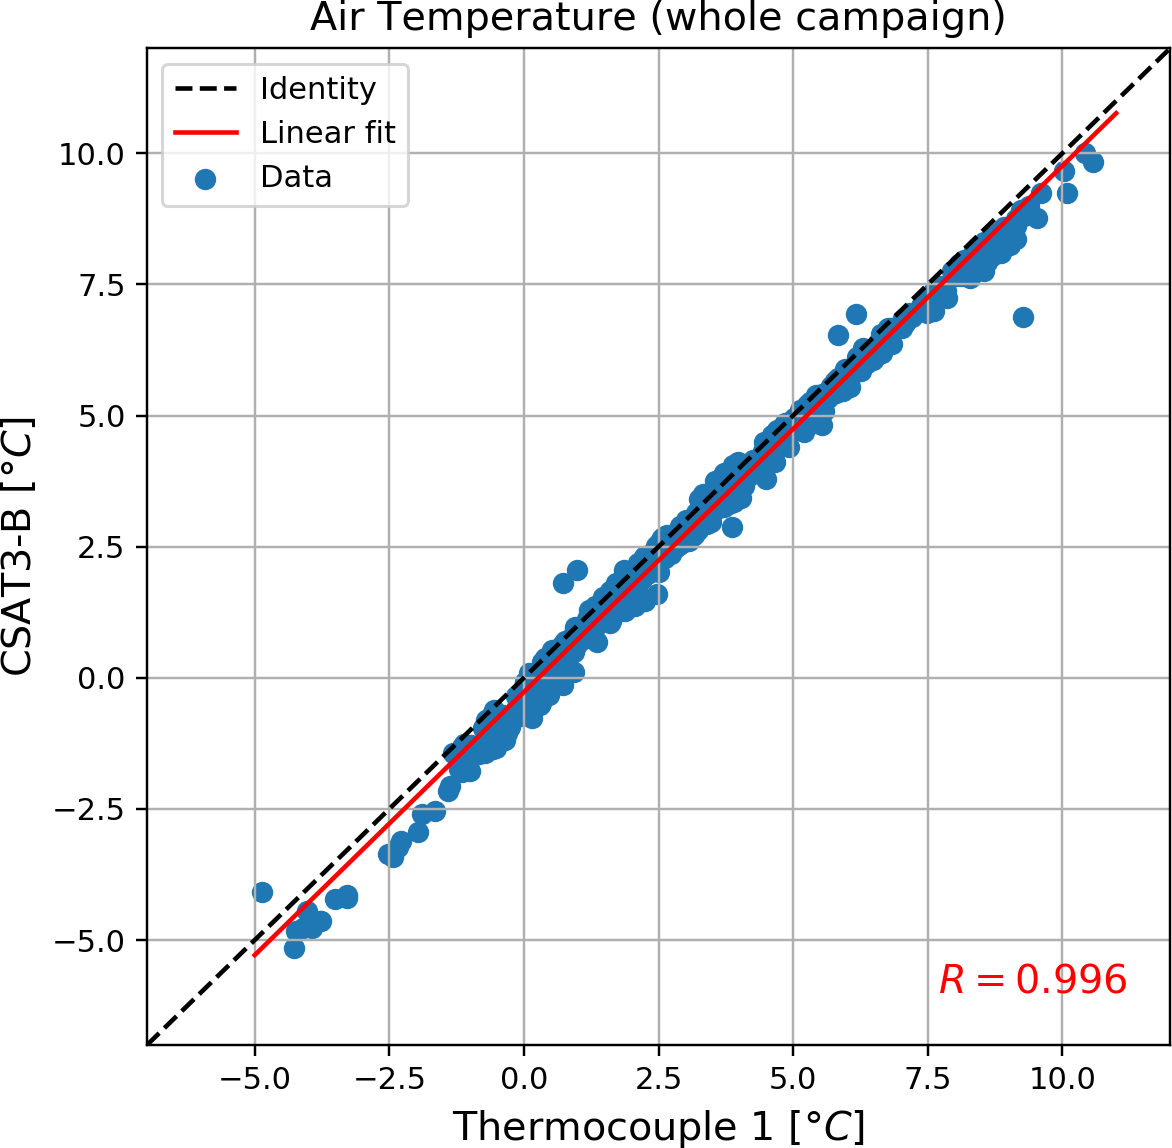
\includegraphics[width=\textwidth]{fig/chapter_4/csat3b_vs_T1.png}
      \label{fig:csat3b_vs_TC1}
    \end{subfigure}
    \quad
    \begin{subfigure}[b]{0.48\textwidth}
        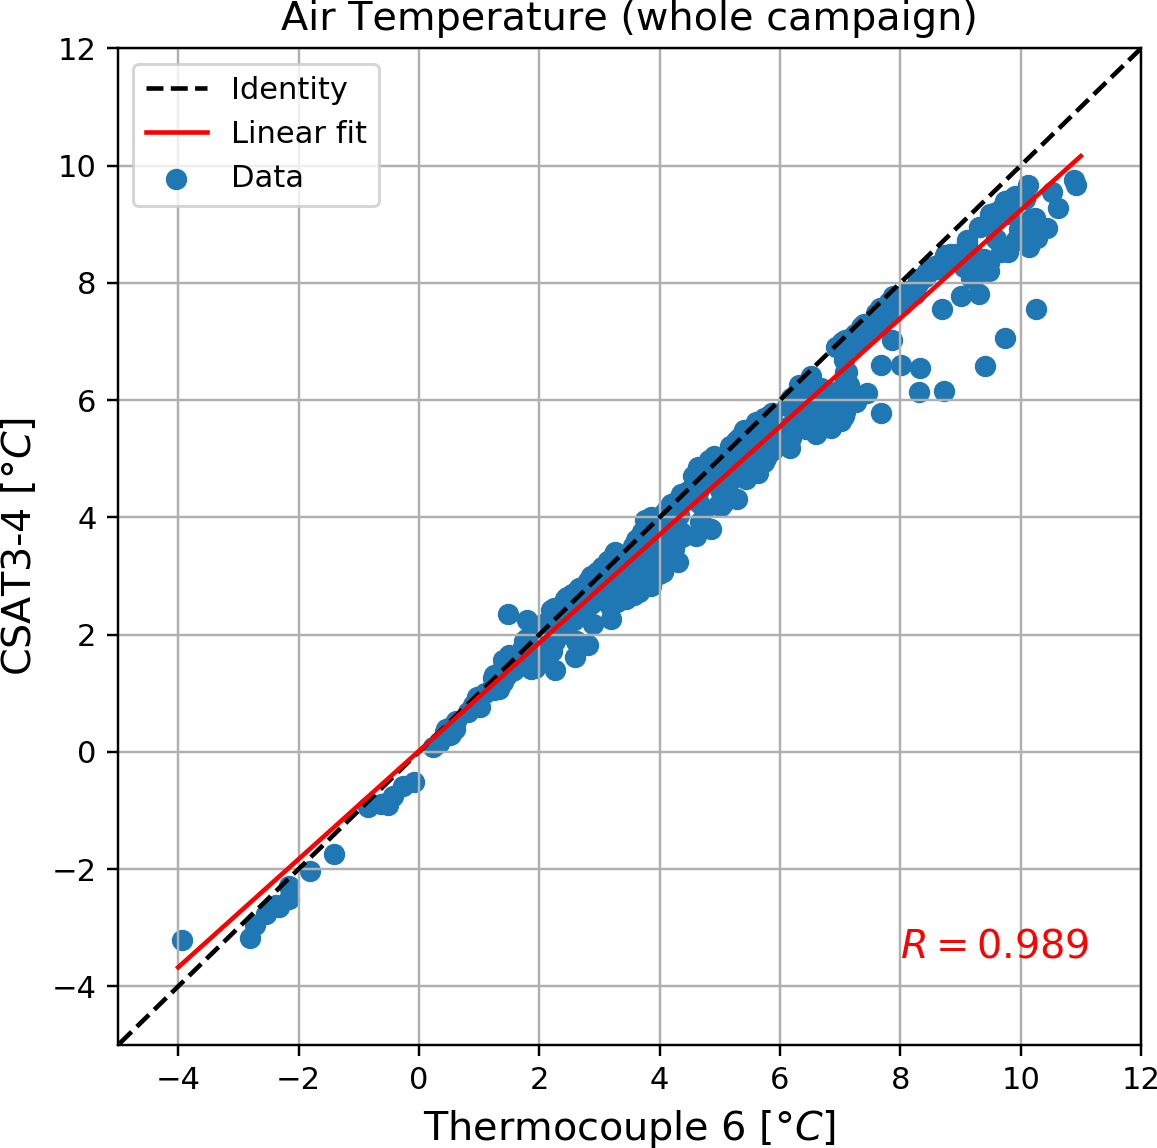
\includegraphics[width=\textwidth]{fig/chapter_4/csat4_vs_T6.png}
        \label{fig:csat4_vs_TC6}
    \end{subfigure}
    \caption{Comparison between the sonic temperature measured with the CSAT3 instruments with a Thermocouple placed at the same vertical level. Each plot has a correlation coefficient, $R$.}
    \label{fig:csat_vs_TC}
\end{figure}

%\section{Temperature gradient}

%Pending (probably not going to put it).

\section{Temperature and wind speed vertical profiles}
For sake of simplicity and because the nights of the 16-17th and 23-24th are similar, in this section we present only the 23-24th night, leaving the results of the 16-17th night for the appendix~\ref{ch:appendix}. 

%\subsection{Night of the 23th to the 24th}

In figure~\ref{fig:18-21_profiles.png} the vertical profiles of the air temperature and the wind speed on a period between 18h00 and 20h30. The air temperature profiles show the measurements done using the Thermocouples (T1 - T10). The wind speed profiles show the measurements done by the CSAT3 and Windsonic 2-D anemometers. At the right of the figure is possible to see a polar plot with the wind direction (point into the direction where the wind is coming to the instrument). The $0 \degree$ angle is aligned with the North. Each level of different radius corresponds to the value of a certain instrument: closer to the centre is the CSAT3-B (B), and in the outer radius, the Windsonic 2-D No.0 (WS0). Globally, the colour of the curves and points on the three subfigures correspond to the values at the same hour, which allows us to identify the temperature, the wind speed and the direction of the profile at a particular time.

\begin{figure}[!ht]
    \centering
    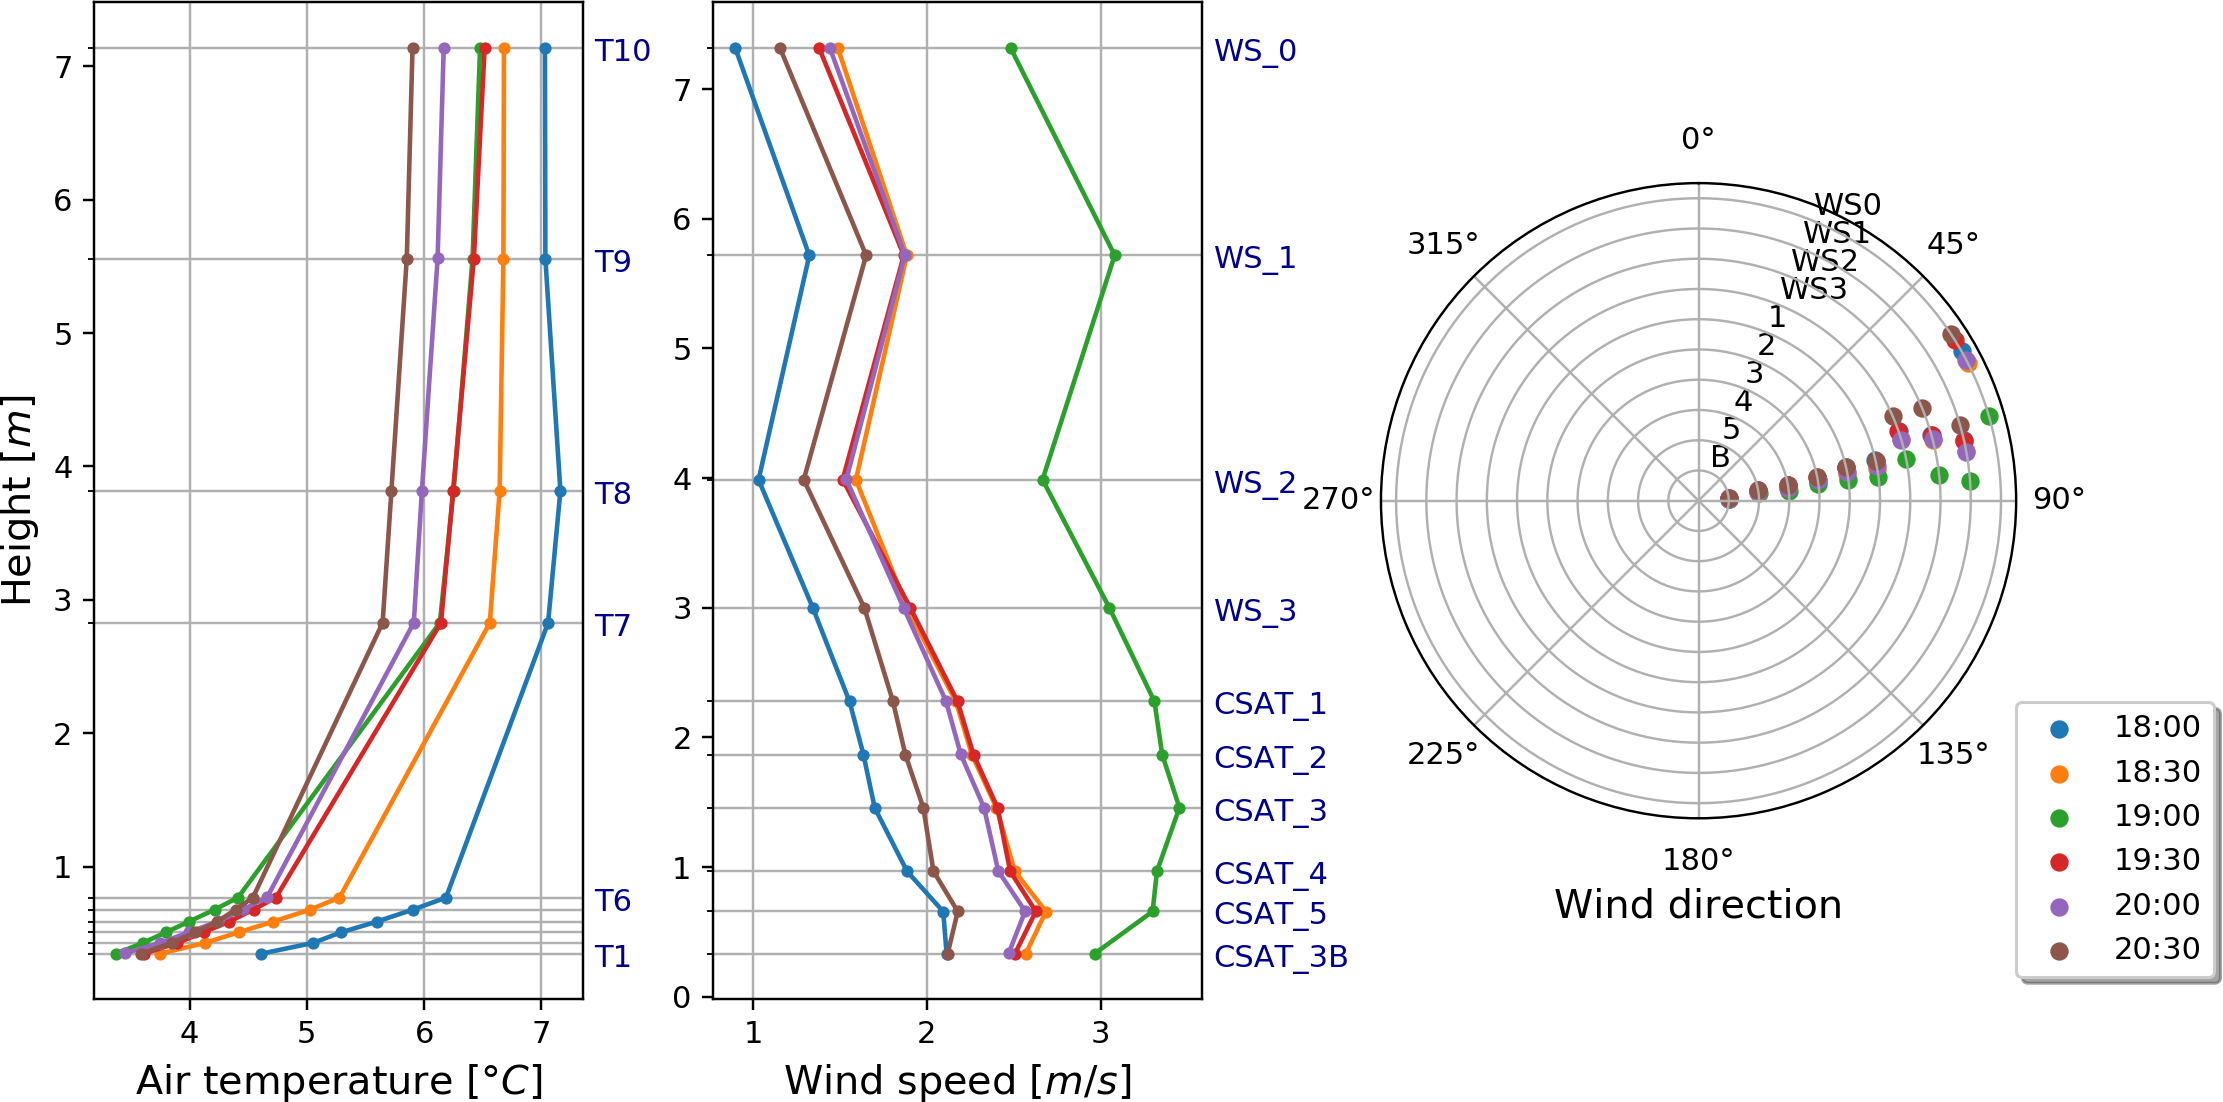
\includegraphics[width=1\textwidth]{fig/chapter_4/23-24/18-21_profiles.png}
    \caption{Temperature and wind speed vertical profiles, with the corresponding wind direction at a particular time, for the period between 18h00 and 20h30 on the night of the 23-24th.}
    \label{fig:18-21_profiles.png}
\end{figure}

Similar to the previous figure, on figure~\ref{fig:21-23_profiles.png} we show the vertical profiles of air temperature and wind speed for the period between 21h00 and 23:30. 

\begin{figure}[!ht]
    \centering
    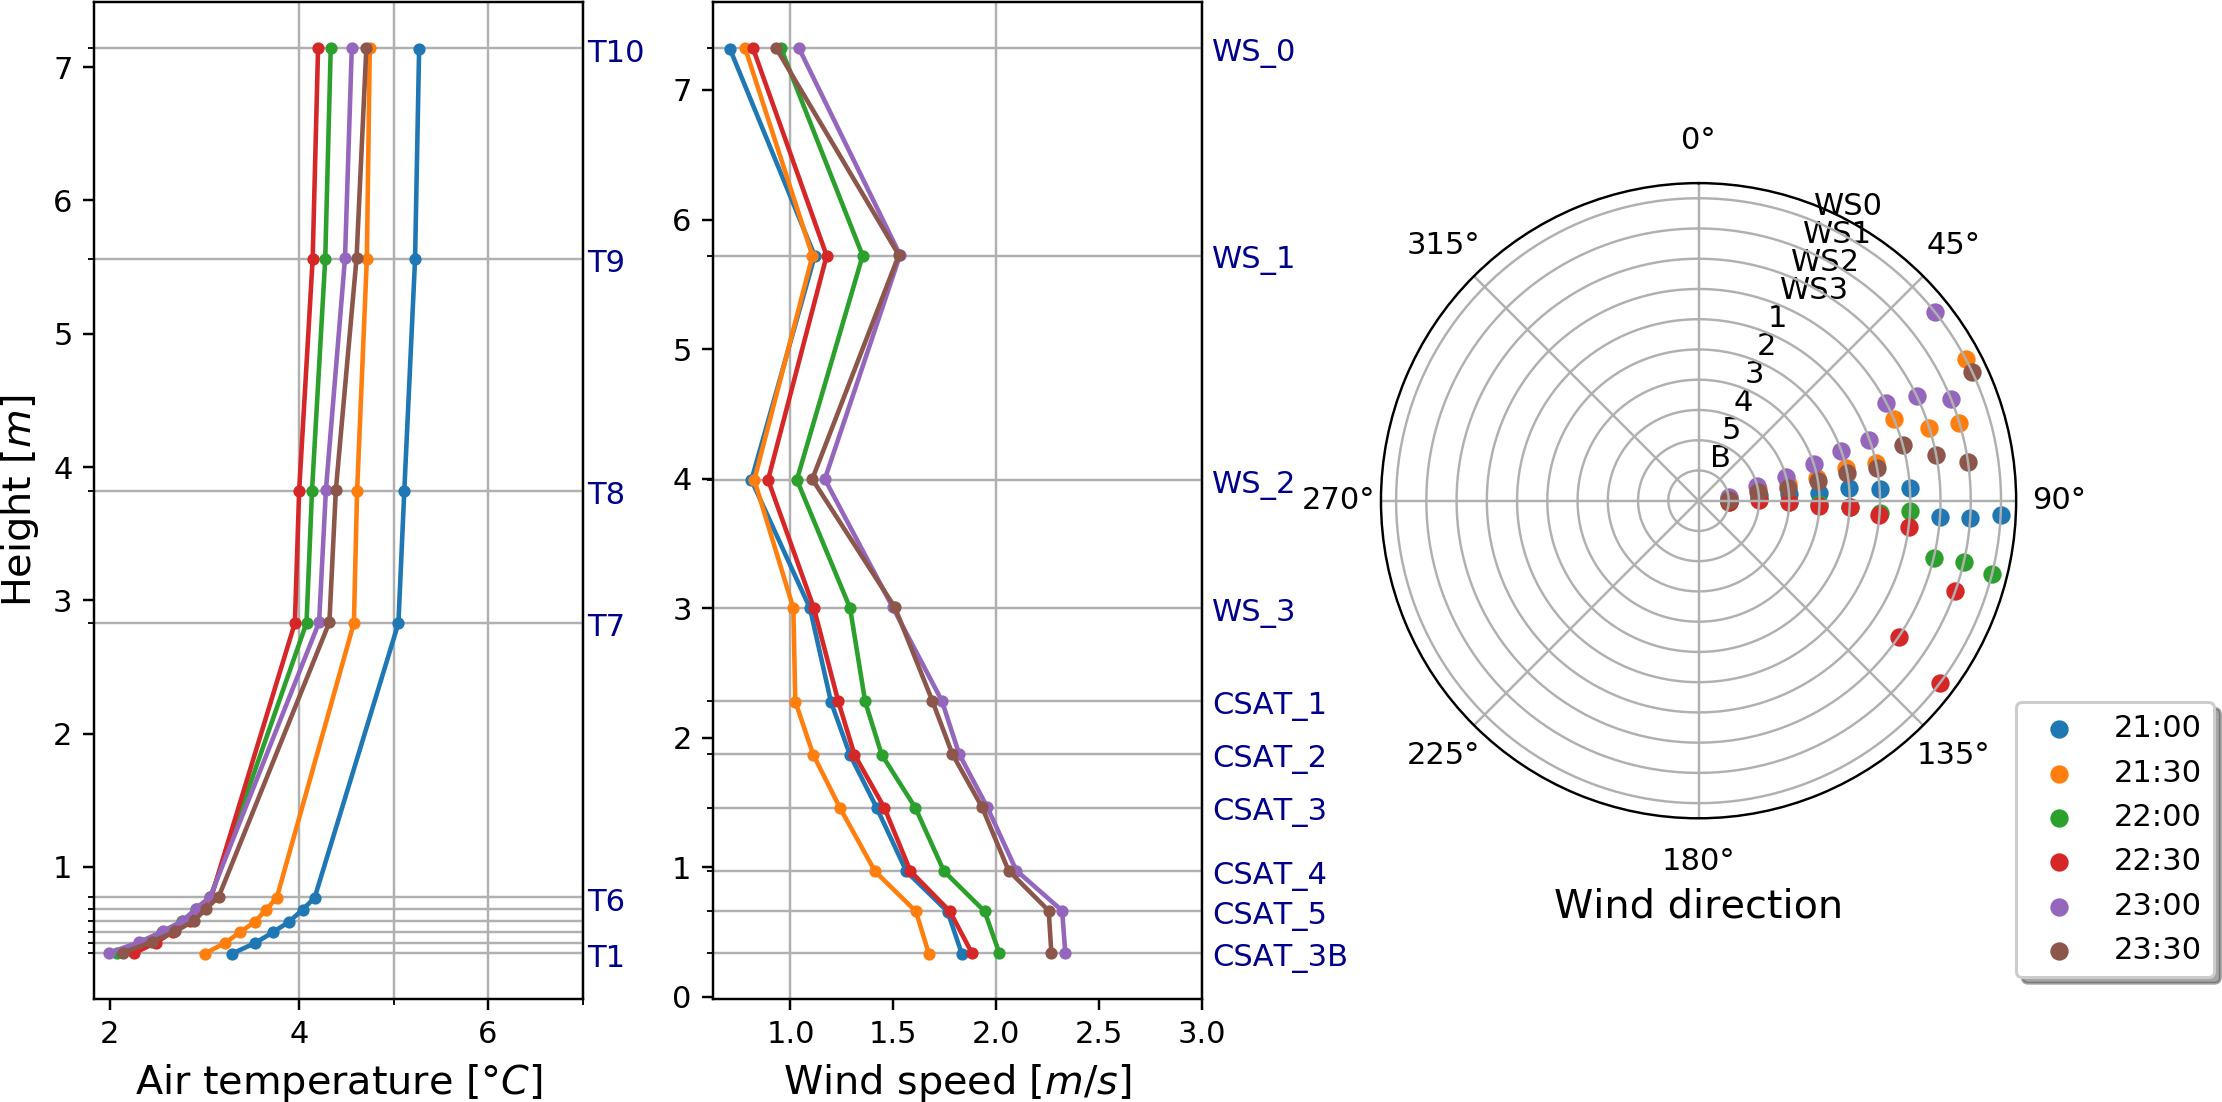
\includegraphics[width=1\textwidth]{fig/chapter_4/23-24/21-23_profiles.png}
    \caption{Temperature and wind speed vertical profiles, with the corresponding wind direction at a particular time, for the period between 21h00 and 23h30 on the night of the 23-24th.}
    \label{fig:21-23_profiles.png}
\end{figure}

\section{Verical fluxes and TKE}

In this section, we present the momentum flux ($\tau$), the sensible heat flux ($H$) and the Turbulent Kinematic Energy ($TKE$), computed with a five minutes average for the night of the 23-24th of February. As in the previous section, the fluxes for the night of the 16-17th can be found in the appendix~\ref{ch:appendix}.

In figure~\ref{fig:23-24_flux_series} we show the time series from the three fluxes between the 20h00 up to 23h30. These fluxes are only shown for the CSAT3 anemometers, and that is because these instruments measure simultaneously the temperature and the three components of the wind, allowing us to compute the vertical fluxes. The time series shows the variation of these quantities over time but is difficult to identify the value that corresponds to a particular instrument.

\begin{figure}[!ht]
    \centering
    \begin{subfigure}[b]{0.65\textwidth}
        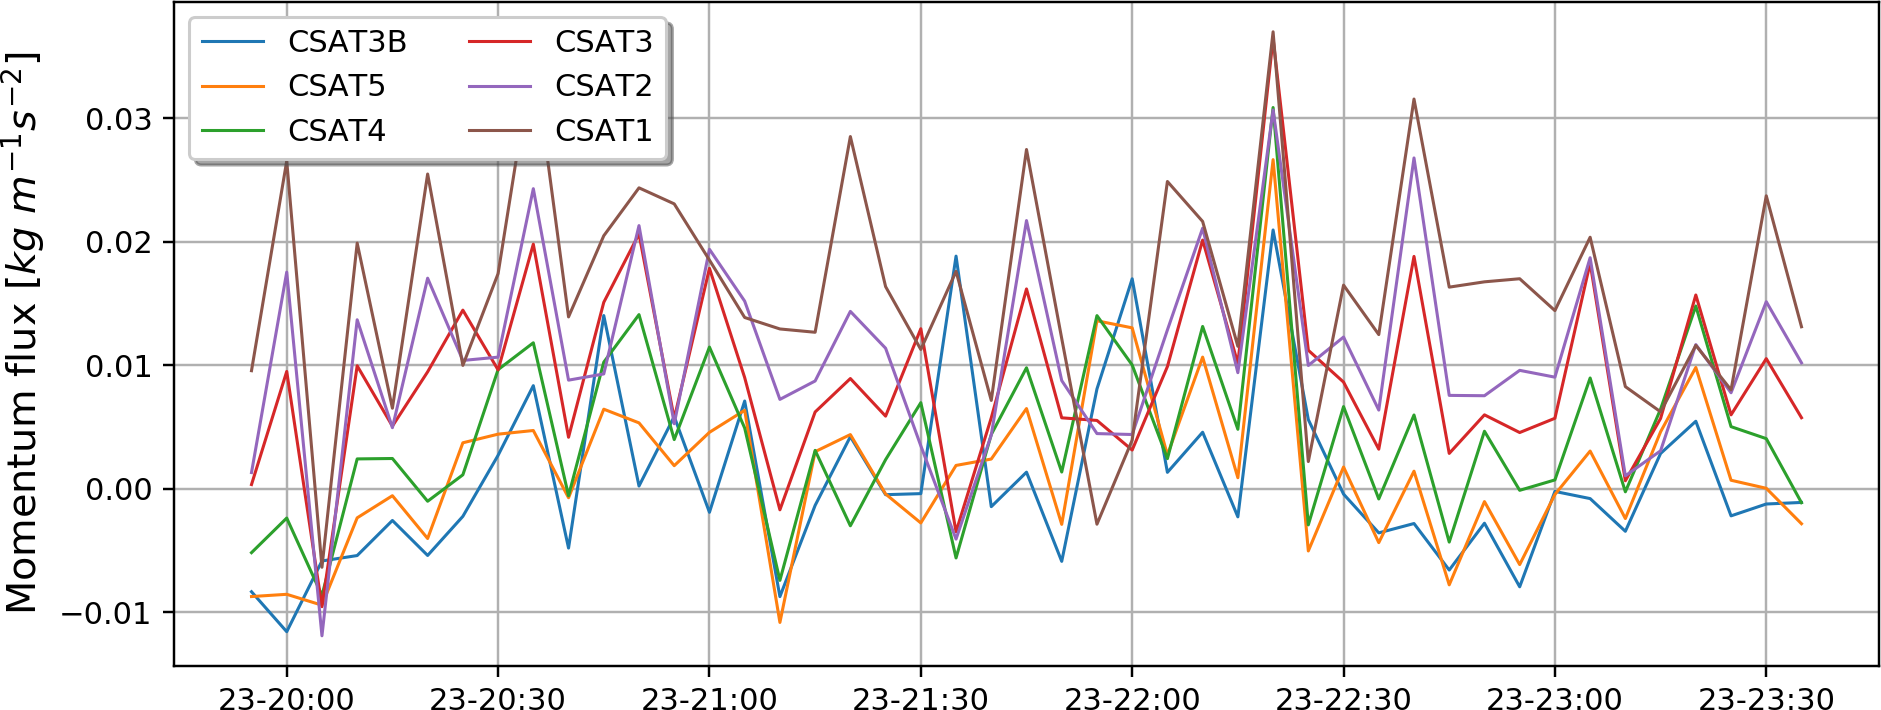
\includegraphics[width=\textwidth]{fig/chapter_4/23-24/Tau_23-24.png}
      \label{fig:Tau_23-24}
    \end{subfigure}
    \begin{subfigure}[b]{0.65\textwidth}
        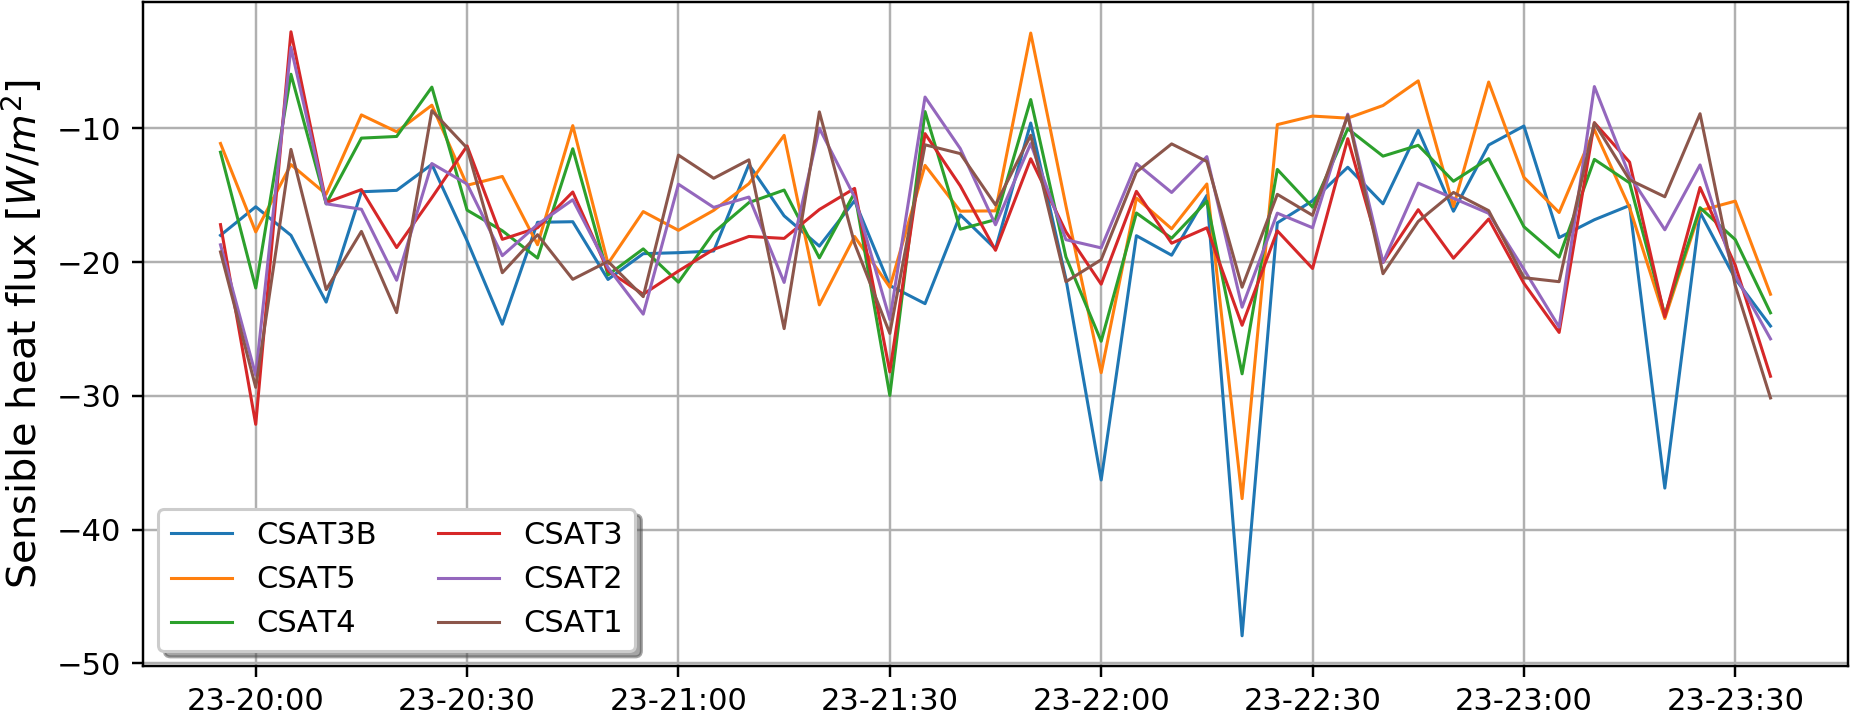
\includegraphics[width=\textwidth]{fig/chapter_4/23-24/H23-24.png}
        \label{fig:H_23-24}
    \end{subfigure}
    \begin{subfigure}[b]{0.65\textwidth}
        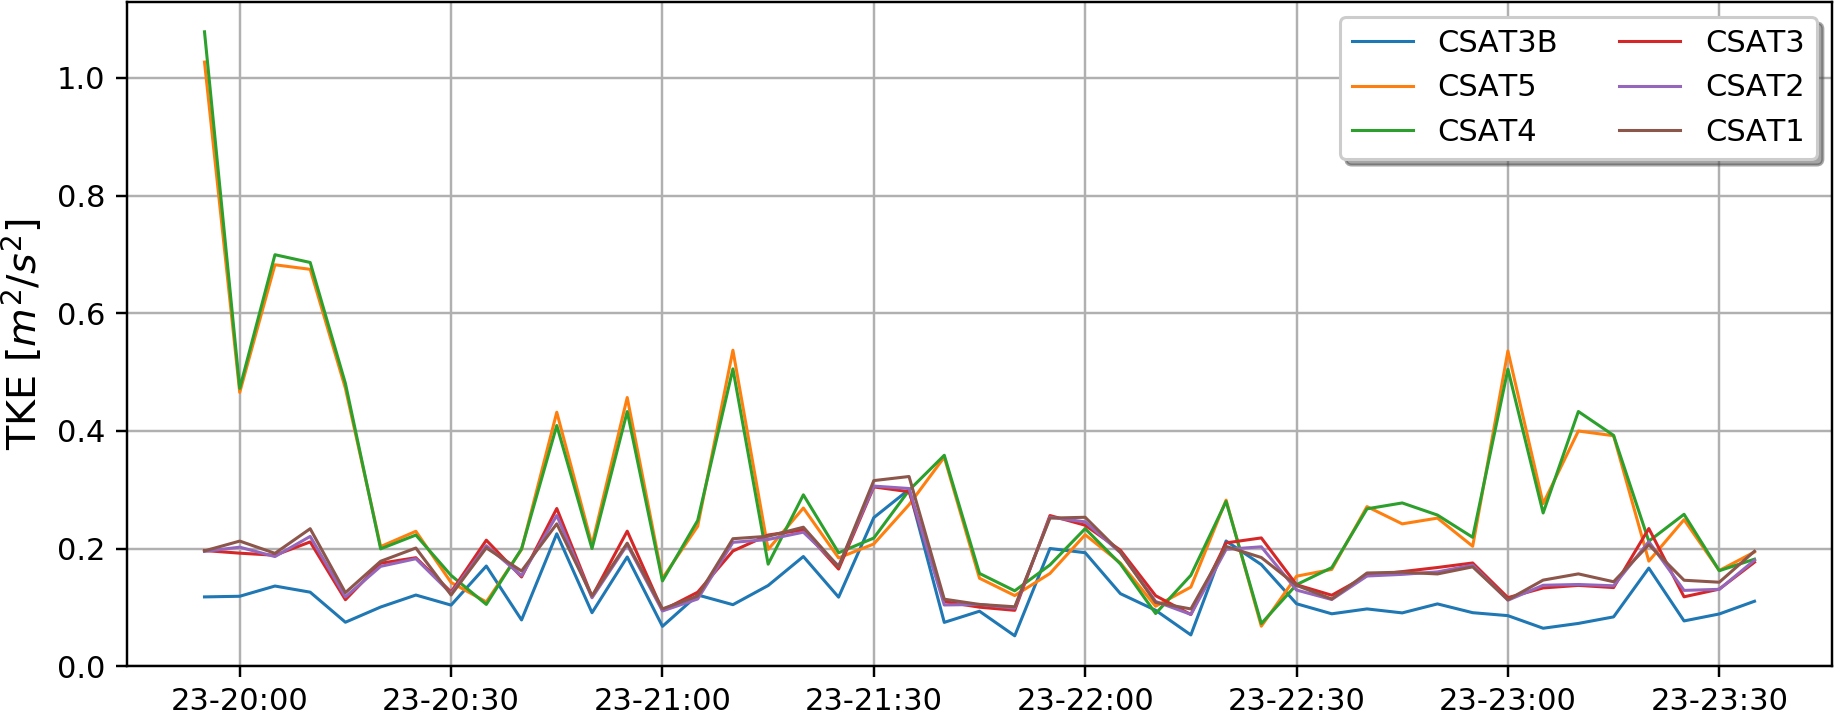
\includegraphics[width=\textwidth]{fig/chapter_4/23-24/TKE23-24.png}
        \label{fig:TKE_23-24}
    \end{subfigure}
    \caption{Time series of the momentum flux (upper figure), temperature flux (middle figure) and Turbulent Kinetic Energy (lower figure).  }
    \label{fig:23-24_flux_series}
\end{figure}

To improve the analysis we selected a particular hour, based on the 30 minutes average profiles, that had a clearly defined maximum in the wind speed and with a wind direction coming from $90\degree$. With this in mind, we selected two hours during the night and plotted the vertical profiles. The times were 20h00 and 23h00. In figure ~\ref{fig:vert_prof_a}, we show four profiles around 20h00, where at the left is the momentum flux as $\tau$, the second panel corresponds to the sensible heat flux $H$, the third is the Turbulent Kinetic Energy ($TKE$) and the fourth one is the wind speed profile ($u$). 

\begin{figure}
    \centering
    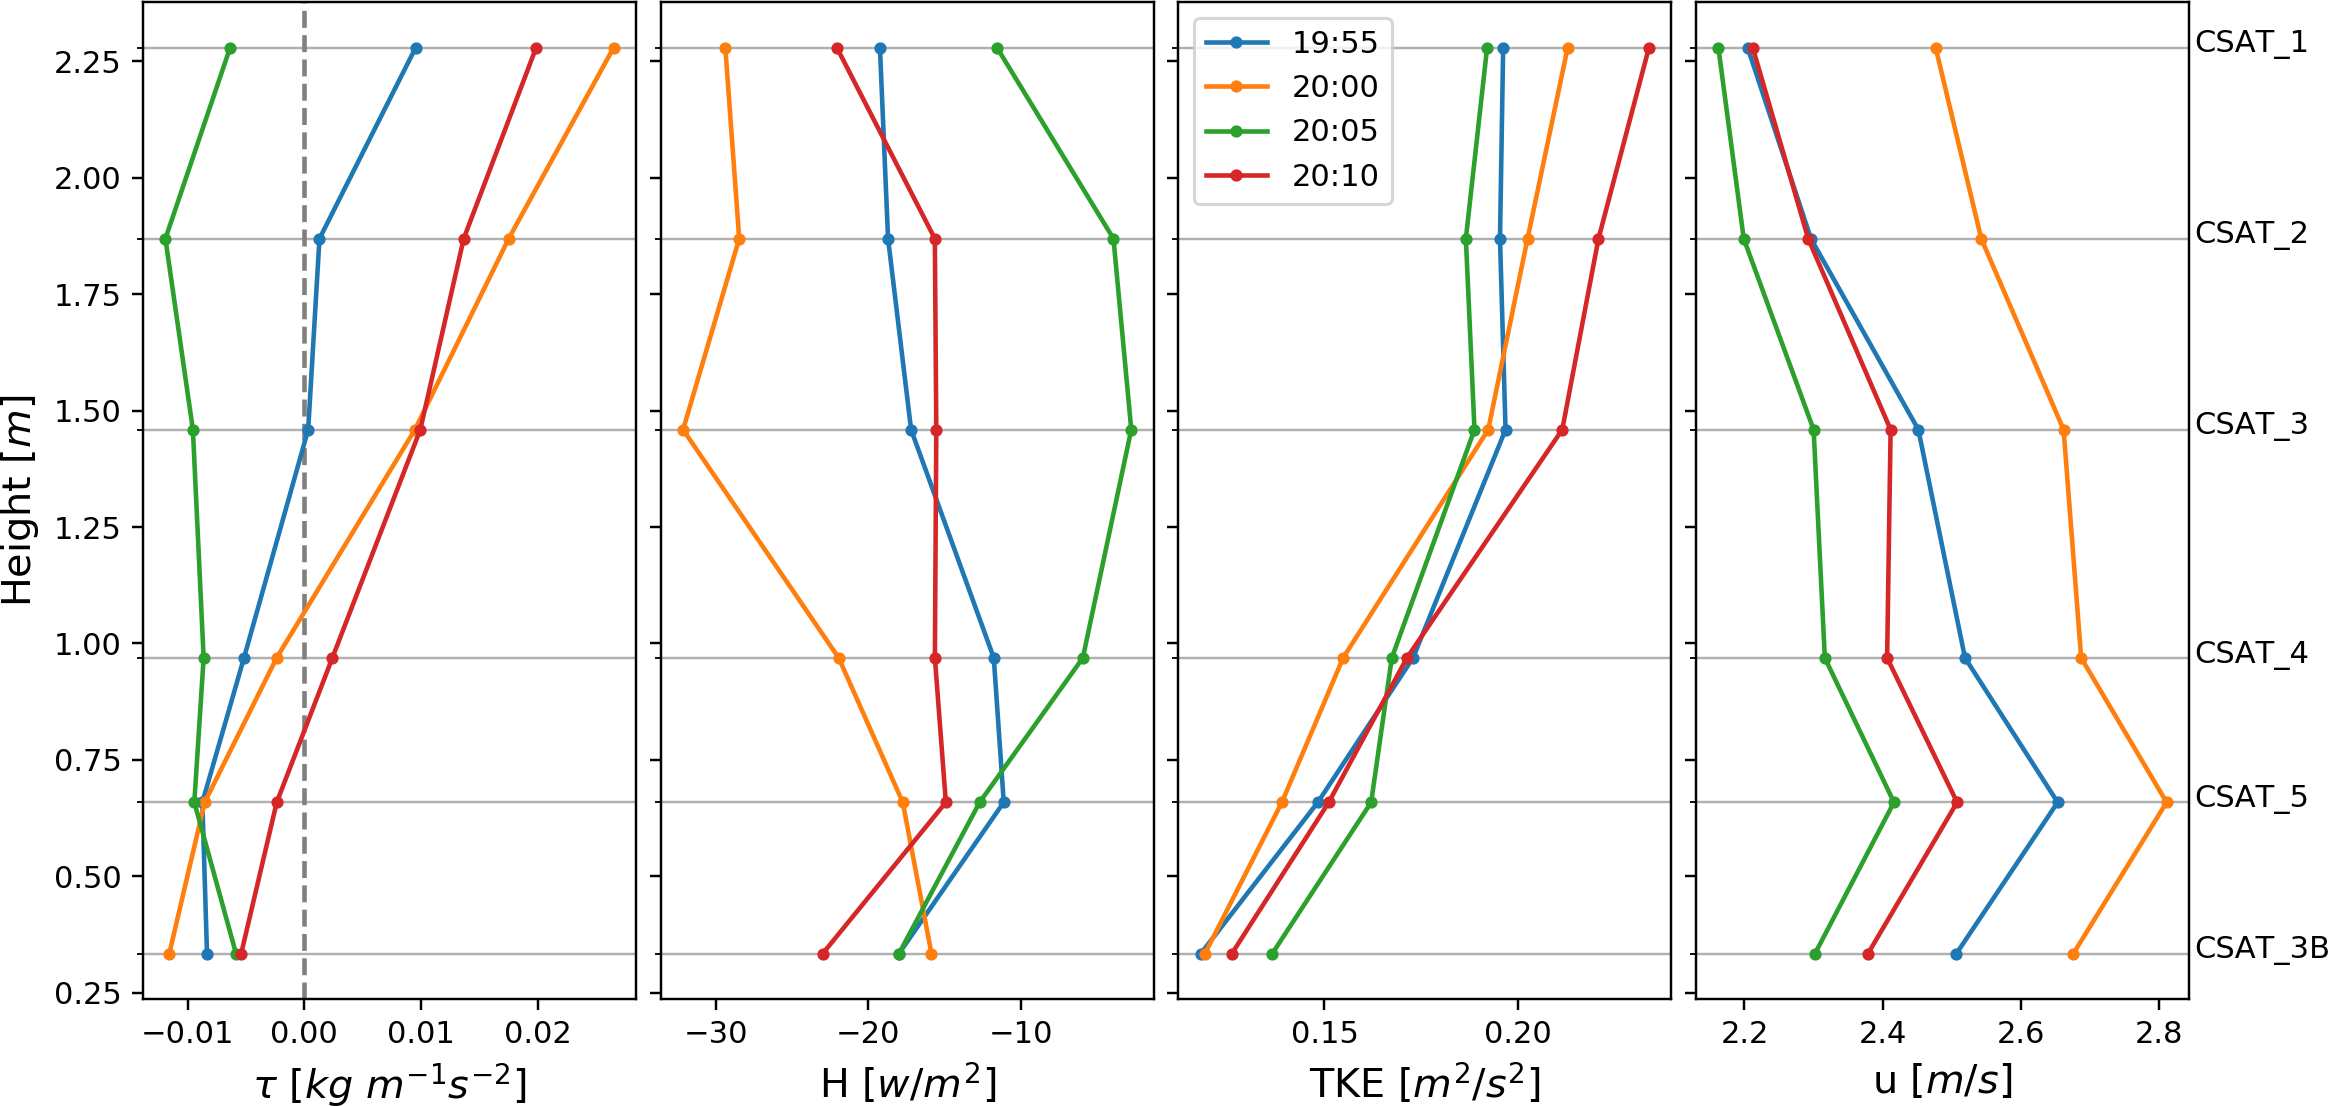
\includegraphics[width=1\textwidth]{fig/chapter_4/23-24/vert_prof_a_speedmax.png}
    \caption{Caption}
    \label{fig:vert_prof_a}
\end{figure}

In the same manner, in figure~\ref{fig:vert_prof_b} we show the profiles for the flux, the TKE and the winds speed around 23h00. 

\begin{figure}
    \centering
    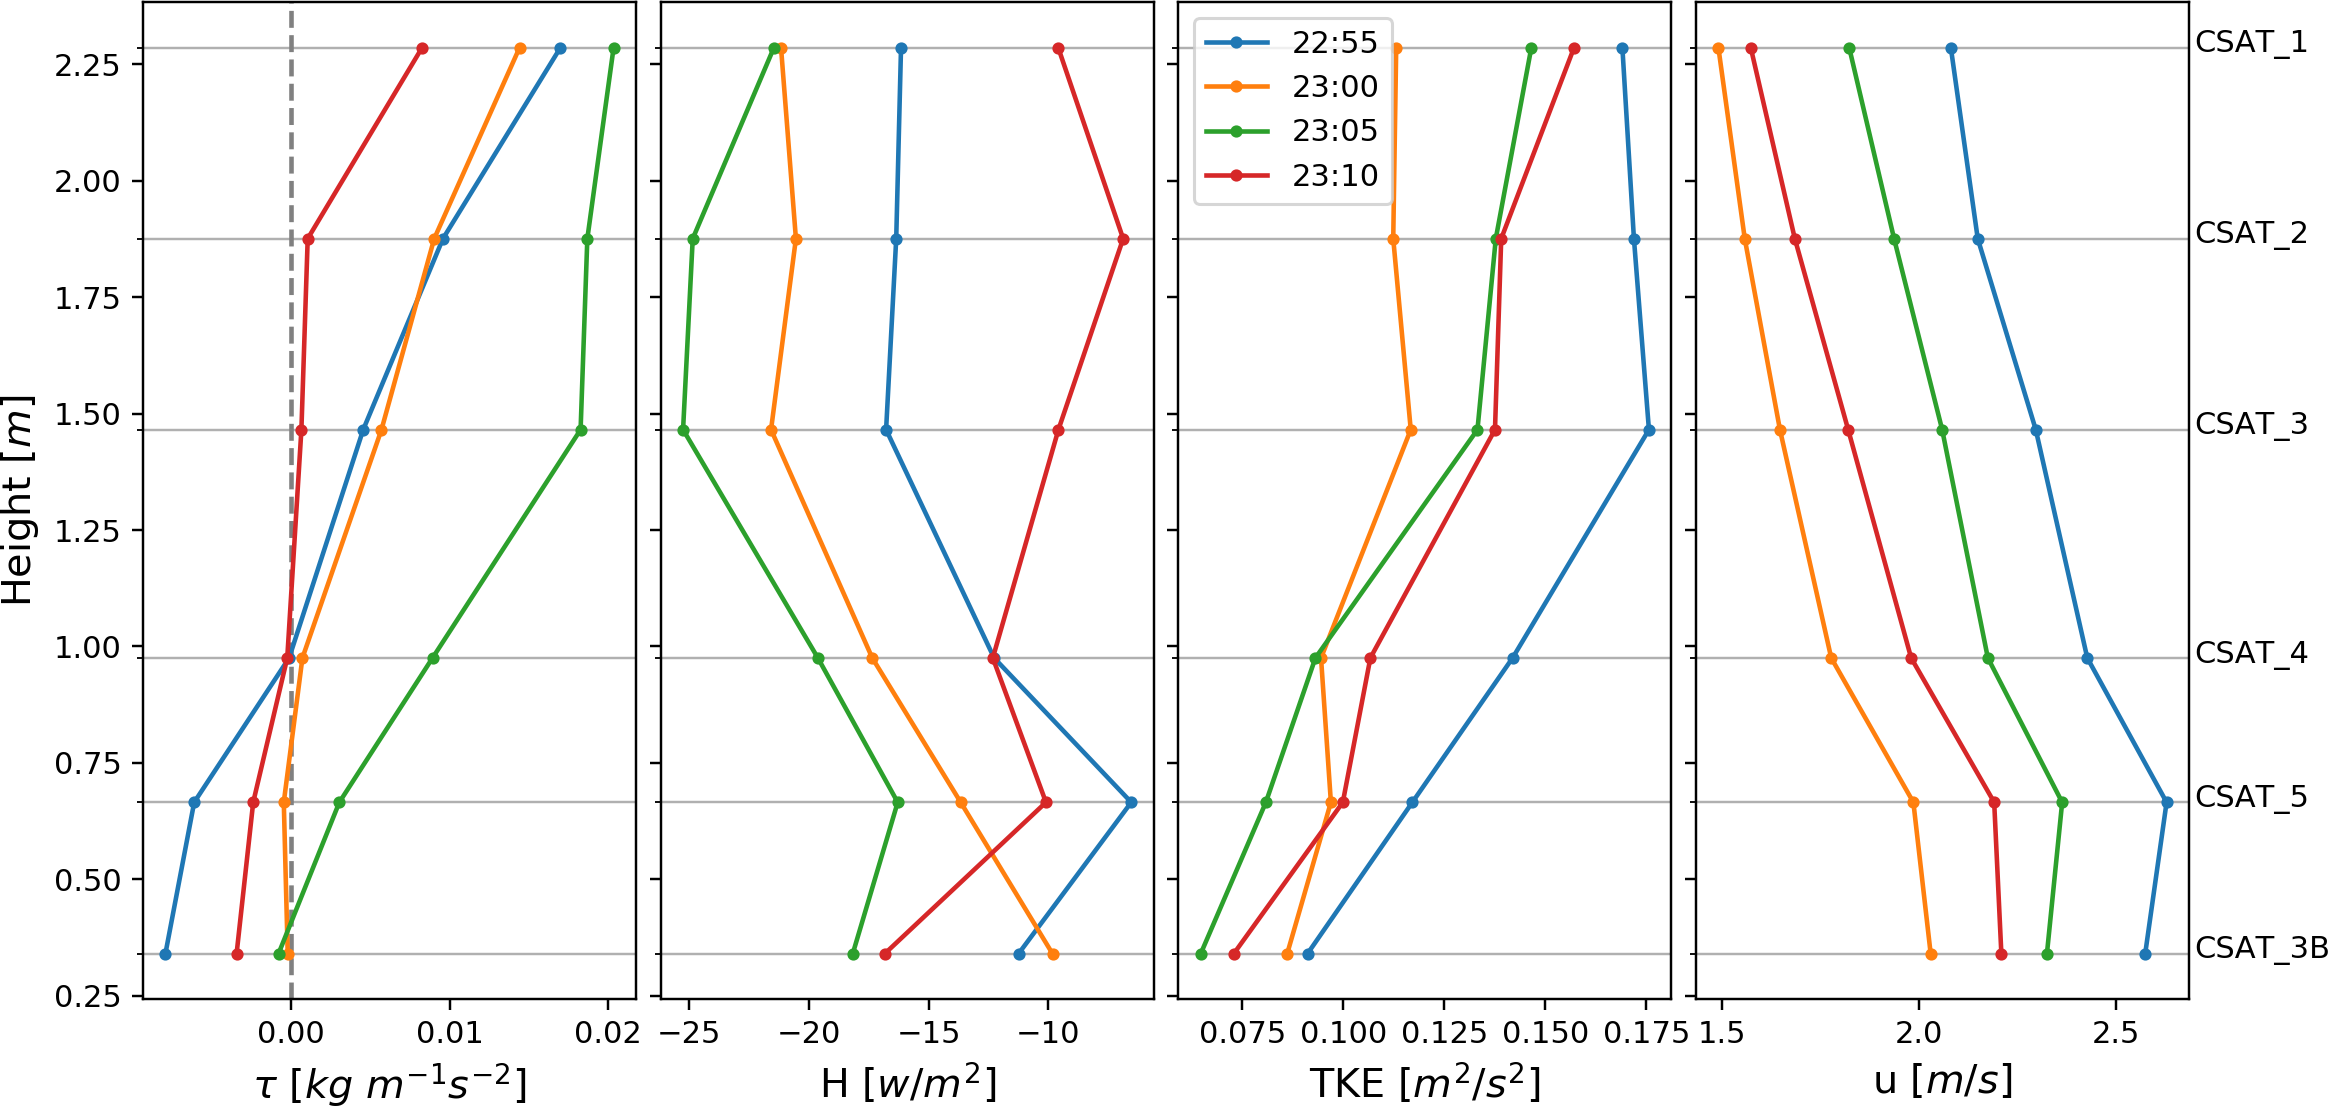
\includegraphics[width=1\textwidth]{fig/chapter_4/23-24/vert_prof_b_speedmax.png}
    \caption{Caption}
    \label{fig:vert_prof_b}
\end{figure}